\documentclass[11pt]{amsart}

\usepackage{physics}
\usepackage{graphicx}
\usepackage{amsmath}
\usepackage[utf8]{inputenc}
\usepackage{hyperref}

\title[FYS3120: Problem Set 1]{Generalised Coordinates \\ \hrulefill\small{ FYS3120: Problem Set 1 }\hrulefill}
\author{Sebastian G. Winther-Larsen}
\date{\today}

\begin{document}

\maketitle

\tableofcontents

\section{Degrees of Freedom and Generalised Coordinates}

Figure \ref{fig:mechanicalsystems} shows four mechanical systems, each of which can be studied and a number of degrees of freedom as well as a set of generalised determined. In general, the number of degrees of freedom and the number of generalised coordinates needed to describe the system are the same, determined by the following formula:
\begin{equation}
\label{eq:dof}
d = N - M,
\end{equation}
where $N$ is the number of coordinates needed to describe every particle or object in the system accuratelym and $M$ is the constraints in the system. $N$ can sometimes be broken down to $N = Dn$, where $D$ is the number of dimension and $n$ is the number of particles.

\subsection{Pendulum with moving anchor}
Subfigure a in figure \ref{fig:mechanicalsystems} shows a pendulum attached to a moving block, which in turn is attached to a spring. The block can in this two-dimensional system be described by two translational coordinates and one rotational coordinates. The mass at in the pendulum is rotationally symmetrical and can therefore be described by two translational coordinates. This gives five, $N=5$, coordinates in total. 

The block is attached to a spring and can only move in a horizontal direction. Furthermore, the block lies flat and is constrained from tilting. The pendulum must remain a fixed distance from its anchoring point at the center of the block. This gives three, $M=3$, constraints in total, and $d = 5 - 3 = 2$ degrees of freedom.

An appropriate set of generalised coordinates is the horizontal position $x$ of the block and the angle $\theta$ the pendulum makes with a vertical line through its anchoring point.

\begin{figure}
	\centering
	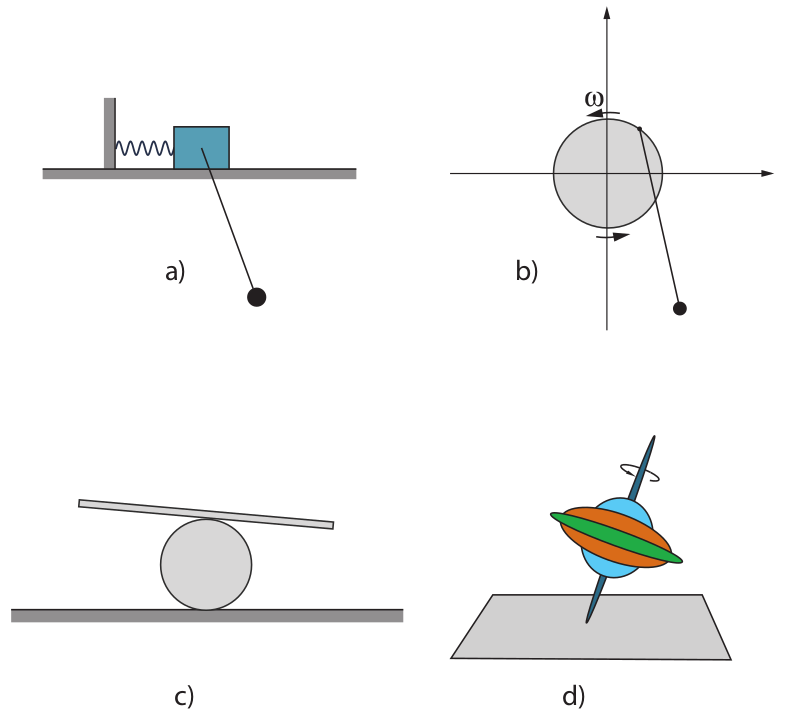
\includegraphics[width = 0.7\textwidth]{./figures/problem1.png}
	\caption{Four mechanical systems}
	\label{fig:mechanicalsystems}
\end{figure}

\subsection{Pendulum attached to spinning disk}
Subfigure b in figure \ref{fig:mechanicalsystems} shows a pendulum anchored to a rotating disk, with a set angular velocity $\omega=\dot{\theta}$. Attached to this disk is a pendulum. To describe the disk, two translational coordinates and one rotational coordinate ($\theta$). The mass of the pendulum is a point in two dimensions, thus two translational coordinates are needed to describe it. This analysis yields five, $N=5$, coordinates in total. 

The  disk is mounted fast, and does not move horizontally or vertically. It rotates with a fixed speed, such that $\theta = \omega t$. The mass at the end of the pendulum can be no more than the length of the string away from its anchoring point. This adds up to four, $M=4$, constraints in total and $d = 5-4=1$ degrees of freedom.

A good pick for a generalised coordinate for this system is the angle $\phi$ that the pendulum makes with a straight vertical line through its anchoring point.

\subsection{Makeshift see-saw}
Subfigure c in figure \ref{fig:mechanicalsystems} shows a straight rod which can tilt without sliding on top of a cylinder, which can roll on a horizontal plane. The cylinder requires two translational coordinates and one rotational coordinates ($\phi$) in order to be described. The rod requires the same, for at total of six, $N=6$, coordinates.

The cylinder can only move horizontally, such that $\Delta y=0$ and is required to roll without slipping, such that $\delta x = s = r\phi$. That is, the length is has rolled is the arc length computed from the change in angle. This will move the rod a length $2s$ in the same direction. The rod can only be moved horizontally in this manner and cannot move vertically. This will change the pivot point of the rod, around which it can still tilt. This gives two constraints for the cylinder and two for the rod, for a total of four, $M=4$, constraints and $d = 6-4=2$ degrees of freedom.

The horizontal position $x$ of the cylinder, and the angle $\theta$ of the rod makes with a horizontal line are sufficient as a set of generalized coordinates.

\subsection{The dreidel}
Subfigure d in figure \ref{fig:mechanicalsystems} shows a spinning top which moves on a horizontal floor. In order to find the degrees of freedom in this situation, I found it to be easier to find the generalised coordinates first. If the tip of the spinning top is constrained to the same point on the plane on which it is spinning, this is an easy matter. We need to know the angle the top is tilted outwards from a centre axis $\theta$, its angular position about this centre axis $\phi$ and the rotation about its own axis $\omega$. This adds up to three generalised coordinates, and the spinning top must have the same number of degrees of freedom.

\section{Double Atwood's engine}

Figure \ref{fig:atwood} shows a double Atwood's engine\footnote{A regular/single Atwood's engine has only one pulley.} consisting of three masses $m_1 = 4m$, $m_2=2m$ and $m_3=m$, two massless pulleys and two massless ropes of length $l_1$ and $l_2$.

This system can be considered one-dimensional, because the objects can only move vertically. If one fixes the origin at the top of the uppermost pulley, there are three moving parts one must monitor; the three masses and the lower pulley. This translates to four coordinates; $y_1$, $y_2$, $y_3$ and $y_4$ for the three masses and the lower pulley.

The first mass and the lower pulley are constrained such that $y_1 + y_4 = l_1$, and the two lower masses are constrains such that $(y_2 - y_4) + (y_3 - y_4) = l_2$. Coordinates together with constraints give the degrees of freedom $d = 4 - 2 = 2$, which means that one can make do with only two generalized coordinates.

\begin{figure}
	\centering
	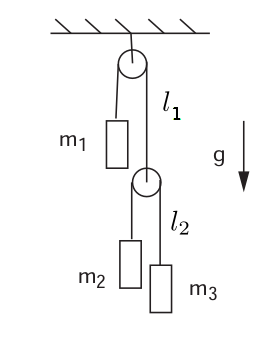
\includegraphics[width = 0.35\textwidth]{./figures/problem2.png}
	\caption{The double Atwood's engine}
	\label{fig:atwood}
\end{figure}

I will pick the distance from the top pulley to the first mass and distance from lower pulley to second mass as generalized coordinates, $q_1=y_1$ and $q_2 = y_2 - y_4$ respectively. This yields 
\begin{align*}
y_1 &= q_1 \\ 
y_4 &= l_1 - y_1 = l_1 - q_1 \\
y_2 &= y_4 + q_2 = l_1 - q_1 + q_2 \\
y_3 &= y_4 + (l_2 - q_2) = l_1 - y_1 + l_2 - q_2 = l_1 + l_2 - q_1 - q_2 
\end{align*}
which is all the cartesian coordinates expressed as functions of the generalized coordinates.

The kinetic energy becomes
\begin{align*}
T 	&= \frac{1}{2}m_1v_1^2 + \frac{1}{2}m_2v_2^2 + \frac{1}{2}m_3v_3^2 \\
	&= \frac{1}{2}m_1\dot{q}_1^2 + \frac{1}{2}m_2(-\dot{q}_1 + \dot{q}_2)^2 + \frac{1}{2}m_3(-\dot{q}_1 - \dot{q}_2)^2 \\
	&= \frac{1}{2}m_1\dot{q}_1^2 + \frac{1}{2}m_2(\dot{q}_1^2 -2\dot{q}_1\dot{q}_2 + \dot{q}_2^2) + \frac{1}{2}m_3(\dot{q}_1^2 + 2\dot{q}_1\dot{q}_2 + \dot{q}_2^2) \\
	&= \frac{1}{2}[ (m_1 + m_2 + m_3)\dot{q}_1^2 + (-2m_2 + 2m_3)\dot{q}_1^2 + (m_2+m_3)\dot{q}_2^2 ] \\
	&= \frac{1}{2}( 7 \dot{q}_1^2 - 2m\dot{q}_1\dot{q}_2 + 3m\dot{q}_2^2)
\end{align*}

The potential energy becomes
\begin{align*}
V 	&= -g( m_1y_1 + m_2y_2 + m_3y_3 ) \\
	&= 
\end{align*}


\end{document}